\documentclass{standalone}
\usepackage{tikz}
\usetikzlibrary{arrows.meta, shapes, calc}

\begin{document}

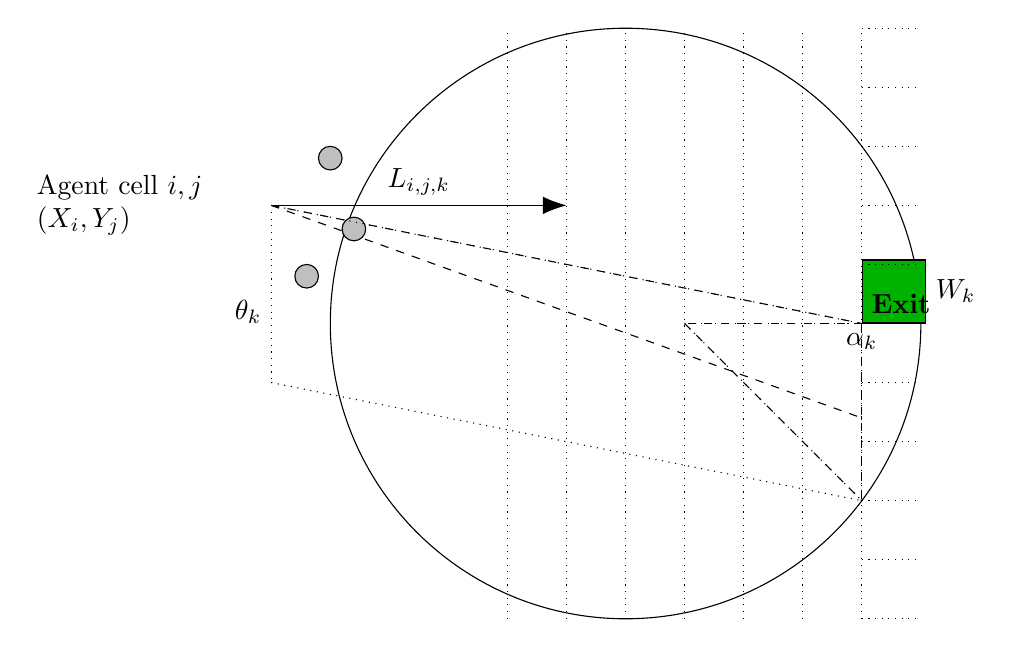
\begin{tikzpicture}[scale=1.5]

% Define coordinates for key points
\coordinate (Agent) at (-3,1);
\coordinate (Exit) at (2,0);
\coordinate (ProjectionPoint) at ($(Exit)+(0,-0.8)$); % Slightly below Exit
\coordinate (CenterCircle) at (0,0);

% Draw the circular boundary (large circle)
\draw (CenterCircle) circle [radius=2.5];

% Draw the dashed lines representing the projection surface
\draw[dashed] (Agent) -- (Exit);
\draw[dashed] (Agent) -- (ProjectionPoint);

% Draw the agent cell
\node[anchor=east, align=left] at ([xshift=-0.5cm]Agent) {Agent cell $i,j$\\$(X_i,Y_j)$};
\node[circle, draw, fill=lightgray, inner sep=0pt, minimum size=0.3cm] at ([xshift=0.5cm,yshift=0.4cm]Agent) {};
\node[circle, draw, fill=lightgray, inner sep=0pt, minimum size=0.3cm] at ([xshift=0.7cm,yshift=-0.2cm]Agent) {};
\node[circle, draw, fill=lightgray, inner sep=0pt, minimum size=0.3cm] at ([xshift=0.3cm,yshift=-0.6cm]Agent) {};

% Draw the exit sign
\node[fill=green!70!black, draw, anchor=south west, minimum width=0.8cm, minimum height=0.8cm, label={right:$W_k$}] at (Exit) {};
\node[below left, white, font=\bfseries] at (Exit.north east) {$\overline{(X_k,Y_k)}$};

% Draw the arrow indicating the viewing direction
\draw[-{Latex[length=3mm]}] (Agent) -- ++(2.5,0) node[midway, above] {$L_{i,j,k}$};

% Draw the angle $\theta_k$
\draw[dotted] (Agent) -- ++(0,-1.5) coordinate (BelowAgent) node[pos=0.6, left] {$\theta_k$};
\draw[dotted] (Exit) -- ++(0,-1.5) coordinate (BelowExit);
\draw[dotted] (Agent) -- (Exit);
\draw[dotted] (BelowAgent) -- (BelowExit);

% Draw the arc indicating $\alpha_k$
\draw[dotted] (Exit) -- ++(-1.5,0) coordinate (LeftExit);
\draw[dotted] (Exit) -- ++(0,-1.5) coordinate (BelowExit);
\draw[dotted] (LeftExit) -- (BelowExit);
\draw[dashed] (Exit) -- ++(-1.5,0);
\draw[dashed] (Exit) -- ++(0,-1.5);
\draw[dashed] (LeftExit) -- (BelowExit);
\node[below, font=\bfseries] at (Exit) {$\alpha_k$};

% Add the vertical dotted lines for reference
\foreach \y in {-2.5,-2,...,2.5} {
    \draw[dotted] (2,\y) -- ++(0.5,0);
}

% Add the horizontal dotted lines for reference
\foreach \x in {-1,-0.5,...,2} {
    \draw[dotted] (\x,-2.5) -- ++(0,5);
}

% Add the final labeling for the exit
\node[above right, font=\bfseries] at (Exit.south west) {Exit};

\end{tikzpicture}

\end{document}